\documentclass[final]{ubb_dolgozat}
\usepackage{definitions}
\usepackage{url}
\sloppy
\frenchspacing

\lstloadlanguages{Java}

\lstset{language=Java}

\submityear{
2016
}
\submitmonthHU{
Július
}
\submitmonthRO{
Iulie
}
\submitmonthEN{
July
}

\titleHU{
Kontroll és egyensúlyozás -- alkalmazás Lego robotnál
}

\titleEN{
Control and balancing -- applied to Lego robots
}

\titleRO{
Control \c{s}i echilibrare -- aplicat la robo\c{t}i Lego
}

\author{
Márton Zete-Örs
}

\tutorHU{
dr. Jakab Hunor,\newline egyetemi adjunktus\\
}
\tutorRO{
Lector dr. Hunor Jakab\\
}
\tutorEN{
Assist prof. dr. Hunor Jakab
}

\begin{document}

\begin{abstractEN}
	
The thesis’ goal is to accomplish a network communication between a mobile application and a MINDSTORMS EV3 two wheeled self balancing robot. To achieve this goal there are two main factors that need to be taken into consideration. Firstly the mobile application that needs to make the communication with the robot, and secondly an algorithm which makes the balancing of the robot possible.

The application and the algorithm which handles the balancing were written in Java. The EV3 control unit is responsible for navigating the robot with the help of the leJOS Linux based framework. The robot remains in a balanced position by using its PID controller and its gyroscope sensor. For it to remain in a balanced state, its velocity, tilt angle and angular velocity needs to approximate to zero. Also its position needs to approximate to zero if it were to remain in a standing balanced position.The PID’s input argument is the error variable which is the difference between the expected value and the current value. In our case we need the error to approximate to zero in order to not lose its balance. Because of this the expected value is always zero. In conclusion the error is made up of four components: the robots tilt angle, angular velocity, velocity and position. By properly modifying these components we can manipulate the robot’s movement.The mobile application connects to the robot through the network and sends eligible commands to it. To accomplish and automated connection between the two components I’ve used the UPnP library, which uses SSDP protocol.

This work is the result of my own activity. I have neither given nor received unauthorized assistance on this work.

\end{abstractEN}

\maketitle

{ \baselineskip 1ex
  \parskip 1ex
  \tableofcontents
}

\chapter{Bevezető}
A szakdolgozat témája robotok egyensúlyozását megvalósító rendszerek tanulmányozása. Ezen rendszereket nevezhetjük zárt vagy nyílt ciklusosnak. Nyílt ciklusos rendszer esetén nincs visszacsatolás, ezért nem megfelelő olyan problémák megoldására, amelyeknél ellenőriznünk kell a rendszer kimenetének eredményét, tehát nem szükséges a visszacsatolás. Egyszerű problémák megoldása esetén használatos. A zárt ciklusos rendszerek visszacsatolással működnek, irányítható a rendszer. Visszacsatolásos működés(\ref{fig:closeLoop} ábra) annyit tesz, hogy a kimenet hatására egy visszajelzést kapunk, amely tulajdonképpen a rendszer bemenete lesz, így a visszajelzés szabályozza a kimenetet és ezáltal komplex feladatok megvalósítására alkalmas.

\begin{figure}[!htb]
	\centering
	\pgfimage[width=0.9\linewidth]{images/close_loop_controller}
	\caption[Zárt ciklusos rendszer működési elve.]
	{Zárt ciklusos rendszer működési elve \href{https://en.wikipedia.org/wiki/Control\_theory}{https://en.wikipedia.org/wiki/Control\_theory}}
	\label{fig:closeLoop}
\end{figure}

Zárt ciklusos rendszerek esetén szabályzó algoritmusról beszélünk, amelyek használata számos technológiában jelen van. Ilyenek közé sorolható a \texttt{Swagway}\footnote{\href{https://swagway.com}{https://swagway.com}} illetve a hasonló szerkezetű és működésű \texttt{Segway}\footnote{\href{http://www.segwaymagyarorszag.com/}{http://www.segwaymagyarorszag.com/}} .

A dolgozat során olyan projekt kerül bemutatásra, amely a LEGO MINDSTORMS EV3\cite{mindstormsEv3} készletből épített kétkerekű egyensúlyozó robot irányítását teszi lehetővé hálózaton keresztül, telefonos alkalmazás segítségével. 

A kétkerekű robot a Gyro Boy\footnote{\href{http://robotsquare.com/wp-content/uploads/2013/10/45544\_gyroboy.pdf}{http://robotsquare.com/wp-content/uploads/2013/10/45544\_gyroboy.pdf}} modell alapján készült el. Főbb komponensei közé sorolható az EV3 vezérlőegység\footnote{\href{http://lego.wikia.com/wiki/45500\_EV3\_Intelligent\_Brick}{http://lego.wikia.com/wiki/45500\_EV3\_Intelligent\_Brick}}, giroszkóp szenzor\footnote{\href{http://shop.lego.com/en-US/EV3-Gyro-Sensor-45505}{http://shop.lego.com/en-US/EV3-Gyro-Sensor-45505}} és a két nagy szervomotor\footnote{\href{http://lego.wikia.com/wiki/45502\_EV3\_Large\_Servo\_Motor}{http://lego.wikia.com/wiki/45502\_EV3\_Large\_Servo\_Motor}}, amelyek egy tengelyen helyezkednek el. Az előbb említett elemekről bővebben szó lesz a \ref{sec:ROBOT:motorok} illetve \ref{sec:ROBOT:szenzorok} fejezetben. Mivel a kerekek egy tengelyen helyezkednek el ezért instabil a szerkezete és könnyen, rövid idő alatt elveszti egyensúlyi állapotát. E probléma megoldására a robot dőlési szöge, szög változásának a sebessége és a robot sebessége 0-hoz kell, hogy tartson, valamint annak érdekében, hogy egy helyben próbálja megtartani egyensúlyát a robot pozíciója is 0-hoz kell közelítsen. 

A probléma megoldására alkalmas a PID\footnote{\href{https://en.wikipedia.org/wiki/PID\_controller}{https://en.wikipedia.org/wiki/PID\_controller}} szabályzó algoritmus használata, amely ipari körökben elterjedt. Viszonylag egyszerű a felépítése, kezelhetősége és az implementálhatósága. A PID szabályzó zárt ciklusos rendszer, melynek a bemeneti értéke a hiba, amely az elvárt érték és az aktuális érték különbsége. Esetünkben mivel 0-t kell közelítsünk annak érdekében, hogy ne veszítse el egyensúlyi állapotát a robot, ezért az elvárt érték örökké 0 lesz, vagyis a hibát négy komponens alkotja: a robot dőlési szöge, szögsebessége, a robot sebessége és pozíciója, amelyek külön-külön súlyozva vannak. A szög és szögsebesség érték meghatározásához a giroszkóp szenzort használjuk és a szervomotorok beépített szenzorjai által lekérhető fordulat szám segítségével számoljuk ki a robot sebességét és pozícióját.

A robot irányításának érdekében szükséges a PID szabályzó algoritmus módosítása és esetleges újabb szabályzók bevezetése annak érdekében, hogy irányítás alatt ne veszítse el az egyensúlyi állapotát. A felhasználónak lehetőséget ad a projekt részeként elkészített Android alkalmazás, hogy hálózaton, socketeken keresztül csatlakozzon a robothoz és az irányításnak megfelelő adatokat továbbítsa. Ezen adatok beviteli módját egy "touch joystick" teszi lehetővé, amellyel négy irányba lehetséges a robot vezérlése. Az adatok védelmét, a tovább bővíthetőséget, illetve a szerializációt a Google Protocol Buffers\footnote{\href {https://developers.google.com/protocol-buffers/}{https://developers.google.com/protocol-buffers/}} biztosítja. A Protocol Buffers platform és nyelvfüggetlen, könnyen kezelhető és gyors. Lehetőséget nyújt az adatok tetszőleges felépítésére, amelynek a forráskódját egy speciális generátor segítségével könnyen kigenerálható. E strukturált adatok írását illetve olvasását biztosítja a generált kód.

Az alkalmazás és a robot közti kapcsolat létrehozásának automatizálására Cling-UPnP(Universal Plug and Play)~\cite{upnp} könyvtárat használjuk, amely SSDP(Simple Service Discovery Protocol)\footnote{\href{https://en.wikipedia.org/wiki/Simple\_Service\_Discovery\_Protocol}{https://en.wikipedia.org/wiki/Simple\_Service\_Discovery\_Protocol}} protokollt használ.

A robot szabályzó algoritmusa Java-ban íródott, amelynek a futtatási környezetét a leJOS firmware biztosítja. Linux alapú  és magába foglalja a JVM-t (Java virtual machine), amely lehetővé teszi, hogy a robot programozható legyen Java-ban. Számos firmware-t fejlesztettek ki annak érdekében, hogy a LEGO MINDSTORMS által fejlesztett vezérlőegységek programozhatóak legyenek magas szinten is. Pár ismert firmware: leJOS\footnote{\href{http://www.lejos.org}{http://www.lejos.org}} José Solórzano hozta létre 1999 végén, nyílt forráskódú, támogatja az objektum orientált programozást, ROBOTC~\cite{robotc} támogatja a C programozást, ev3dev~\cite{ev3dev}, amely a szkript nyelveket támogatja (Phyton, NodeJS, Ruby). 

Az előbb említett firmware-k teszik lehetővé a komplex feladatok megoldását, amelyek nem lehetségesek az EV3 alapértelmezett rendszerével. E rendszerhez a LEGO MINDSTORMS biztosított egy grafikus felületet, amely a kisebb korosztály számára készült, hogy "programozhassák" a saját kezűleg épített robotokat.

A dolgozat négy fejezetből áll. Az első fejezet által betekintést nyerünk a dolgozat témájába. 

A második fejezet röviden bemutatja a LEGO megalakulását, a LEGO MINDSTORMS által kifejlesztett generációkat, majd bemutatja az EV3 készlethez tartozó motorokat és szenzorokat. Tartalmazza azon eszközök részletes leírását, amelyek a projekt során felhasználásra kerültek.

A harmadik fejezet által bemutatásra kerül a PID szabályzó működése és használata e projekt esetén.

A negyedik fejezet célja, hogy bemutassa e szakdolgozat alatt létrehozott projekt működését és az elkészített Android mobil alkalmazást. Valamint a projekt elkészítése során felmerült problémákat, ezek megoldását, illetve lehetséges megoldását.
\chapter{LEGO} \label{ch:ROBOT}

\begin{osszefoglal}
	A fejezet alatt, bemutatásra kerül a LEGO megalakulása, fejlődése. E mellet sor kerül a LEGO MINDSTORMS által kifejlesztett technológiák bemutatása, amelyek közül egy pár felhasználásra kerül a továbbiakban.
\end{osszefoglal}

\section{LEGO megalakulása}\label{sec:ROBOT:lego}
A LEGO története 1932-ben kezdődött,  Ole Kirk Christiansen asztalos vállalkozást alapított Dánia, Billund nevezetű falujában, amely a fa játékok gyártásával foglakozott. 1934-ben vette fel a cég a LEGO nevet, amely a LEG GODT Dán szóból ered. 1947 után kezdtek el műanyagból előállítani játékokat amelyek fő célja az volt, hogy könnyedén egymásba illeszthetőek illetve szétszedhetőek legyenek. Az alapító fia Godtfred Christian lett az igazgató 1958-ban, ekkor alakult meg a ma ismert LEGO vállalat és vezetésével fellendült a cég. Az első számítógép által vezérelt robot 1986-ban jelent meg, amelyet követően 1988-ban a LEGO es az MIT (Massachusetts Institute of Technology) együttműködésével elkezdődött az "inteligens tégla" fejlesztése, mely lehetőséget ad a programozhatóságra.

\section{LEGO MINDSTORMS}\label{sec:ROBOT:mindstorms}
A LEGO első játéka amit forgalmazott Ole Kirk Christians vezetésével a fából készült "LEGO Duck" évekkel később megjelentek a műanyag játékok. Ma már világszerte ismert a LEGO építőjáték, egymással összeilleszthető, kombinálható elemeket tartalmaz így szinte bármi megépíthető belőle és rendkívül hasznos oktatás szempontjából is. 

A LEGO MINDSTORMS, egy programozható robotikai építőkészlet. Lehetőséget ad, hogy megépítsd, programozd és irányítsd a robotot.
1998-ban jelent meg az első generáció az RXC  (Robotic Command eXplorers), akkoriban nagy előrelépés volt mivel képes számítógép nélkül is működni de ma már elavultnak számít.

\subsection{RXC}
Az RXC az elsőgenerácíós LEGO MINDSTORMS. Ma már nem igen használatos, elavult programozható vezérlőegység, mivel csupán 8-bites mikrokontroller és 32KB RAM-al rendelkezik. Tartalmaz három szenzor és három motor csatlakozó port. Ezek mellet egy LCD kijelzőt amin látható volt az akkumulátor töltöttségi szintje, a bemeneti és kimeneti portok állapota illetve egyéb információk megjelenítésere is alkalmas.

\subsection{NXT}
A második generáció, az NXT 2006-ban jelent meg illetve az NXT 2.0 2009-ben amely több építőelemet és szenzort tartalmaz. Több mindenben különbözik az NXT az RXC-hez képest. Szembetűnő esztétikai változások történtek és javítottak a kapacitáson, növelték a portok számát és még más újdonságokat is hozott magával.

Tartalmaz négy szenzor, három motor csatlakozó és egy USB portot. Lehetséges a Bluetooth használata számítógépes csatlakozáshoz, megjelent a grafikus kijelző és tartalmazott egy 8Khz hangszórót. Az NXT 32-bite mikrokontrollerrel, 256KB flash memóriával és 64KB RAM-al rendelkezik.

\subsection{EV3}
A harmadik generáció, az EV3 2013-ban jelent meg, az "EV" evolúciót jelenti és a 3, hogy harmadik generáció. A legfejeltebb programozható építőelem amely kezeli a motorokat, szenzorokat és lehetőséget ad Wi-Fi-n vagy Bluetooth-on keresztül való kommunikációra.

Az EV3 egy ARM9-es nevű processzorral van felszerelve, amely 300Mhz-s, 16MB flash memóriával és 64MB RAM-al rendelkezik. A Linux alapú operációs rendszere nagyban segíti a programozhatóságát. Egy 2.0 USB port van a számítógéppel való kommunikációhoz, aminek átviteli sebessége 480Mbit/s, az SD kártya olvasója 32GB-ot ismer fel. Tartalmaz egy USB portot amely lehetővé teszi, hogy használjunk Wi-Fi dongle-t, ezáltal megkönnyíti a programok kitelepítését, fájlok kezelését és lehetséges a kommunikáció okos készülékekkel is.

Az NXT-hez képest sokat fejlődött, nagyobb a kapacitása, lehetőség van Wi-Fi és SD kártya használatára. Ezek mellet négy szenzor port van három helyett és négy motor csatlakozó port. Nagyobb LCD kijelzőt raktak és a felületén hat gomb van négy helyett, könnyítve az operációs rendszer menüjének kezelését.

\section{Szenzorok}\label{sec:ROBOT:szenzorok}
\section{Motorok}\label{sec:ROBOT:motorok}

\chapter{Egyensúlyozás}\label{ch:EGYENSULY}
\begin{osszefoglal}
E fejezet célja, hogy bemutassa a PID szabályzó algoritmus működését. Emellett sor kelűr az egyensúlyozás működésének leírására, valamint, hogy miként lehet felhasználni ez esetbe a PID szabályzó algoritmust.
\end{osszefoglal}

\section{PID szabályzó algoritmus}\label{sec:EGYENSULY:pid}

A szabályzó rendszereket kétféleképpen nevezhetjük nyílt vagy zárt ciklusosnak.  Nyílt ciklusos rendszerek esetén nincs visszacsatolás, ezért nem megfelelő komplex problémák megoldására. Előnyös a használata kisebb kapacitás esetén, mivel alacsony költségű. A zárt ciklusos rendszerek visszacsatolással működnek, vagyis a rendszer kimenetének hatására visszajelzést kapunk.

A PID\texttt{(Proportional Integral Derivate)} elterjedt zárt ciklusos rendszer, az ipari szabályzó körökben, köszönhetően a viszonylag egyszerű félépítésének és a könnyen kezelhetőségének. Számos felhasználási lehetősége van, ilyenek a nyomás, hőmérséklet, sebesség szabályozás. E szabályzó rendszer bementi értéke az aktuális hiba.

A hibát az elvárt érték és az aktuális érték különbsége határozza meg. Esetünkben az aktuális értékek a következők: robot dőlési szöge, szög változásának sebessége, a robot pozíciója illetve sebessége. Az előbb felsorolt értékek esetén az elvárt értékek, ahhoz, hogy a robot egyensúlyi állapotba maradjon, 0-hoz kell közelítsenek.

A szabályzó kimeneti értéke a motorokra leadott erő. Esetünkben tehát a visszacsatolás az előbb felsorolt négy értékben nyilvánul meg, mivel a kerekre leadott erő befolyásolja ezen értékeket.

A PID, mint a nevéből is látható három tagból tevődik össze: P \texttt{(Proportional)} az arányos tag, I \texttt{(Integral)} a hibák integrált tagja és a D \texttt{(Derivate)} a hibák időbeli változásának derivált tagja. Abban az esetben ha az előbb felsorolt tagok közül nem veszünk figyelembe minden tagot, akkor a következő szabályzókról beszélhetünk: P, PI és PD.

PID szabályzó matematikai képlete: $$u(t)=K_{P}e(t)+K_{I}\int e(t)dt+K_{D}\frac{d}{dt}e(t),$$ ahol $t$ jelöli az időt, $e(t)$ a bemeneti hibát, illetve az $u(t)$ a kimenet. A $K_{P}, K_{I}, K_{D}$ paraméterek rendre az arányos, az integrált és a derivált tagok súlya, amelyek meghatározzák a szabályzó érzékenységét és teljesítményét.

Kizárólag az arányos tag használata esetén a szabályzó rendszer olyan eseteknél használható, ahol megengedett egy bizonyos nagyságú hiba kimenetben miután a rendszer stabilizálódott. Az arányos tag paramétere a $K_{P}$, amely egy konstans érték, ha túl nagy instabil rendszert eredményez.

Az integrált tag önmagában nem használható mint az arányos tag. Az integrált tag esetén a hibák összege mind addig változik míg az arányos tag nulla nem lesz. Tehát a feladata egy pontosabb és precízebb szabályzó rendszer biztosítása. Mivel kód szinten nem valósítható meg az integrálás, ezért a következő képlet segítségével közelítsük meg:$$u(t)=K_{I}\cdot\sum e(t),$$ ahol az előbbihez hasonlóan $K_{I}$ konstans.

A derivált tag értéke arányos a hiba változási sebességével. Feladata a hirtelen változások késleltetése, ezáltal egy stabilabb rendszert biztosítva. Ez esetben is felmerül az előbb említett probléma, ugyanis kód szinten a deriválás sem valósítható meg ezért a következő képlettel közelítsük meg:$$u(t)=K_{D}\cdot (e(t) - e(t-1),$$ ahol szintén a $K_{D}$ konstans.

A \ref{pidFig} ábrán látható a PID szabályzó tagjainak változása egy teszt esetén. Jól látható az ábrán, hogy a derivált tag ellentétes előjelű az arányos taghoz viszonyítva, ennek köszönhetően a hirtelen változások késleltetve lesznek. Az integrált tag és az arányos tag esetén jól látható, hogy hasonló oszcillációt végeznek.

\begin{figure}[h]
	\centering
	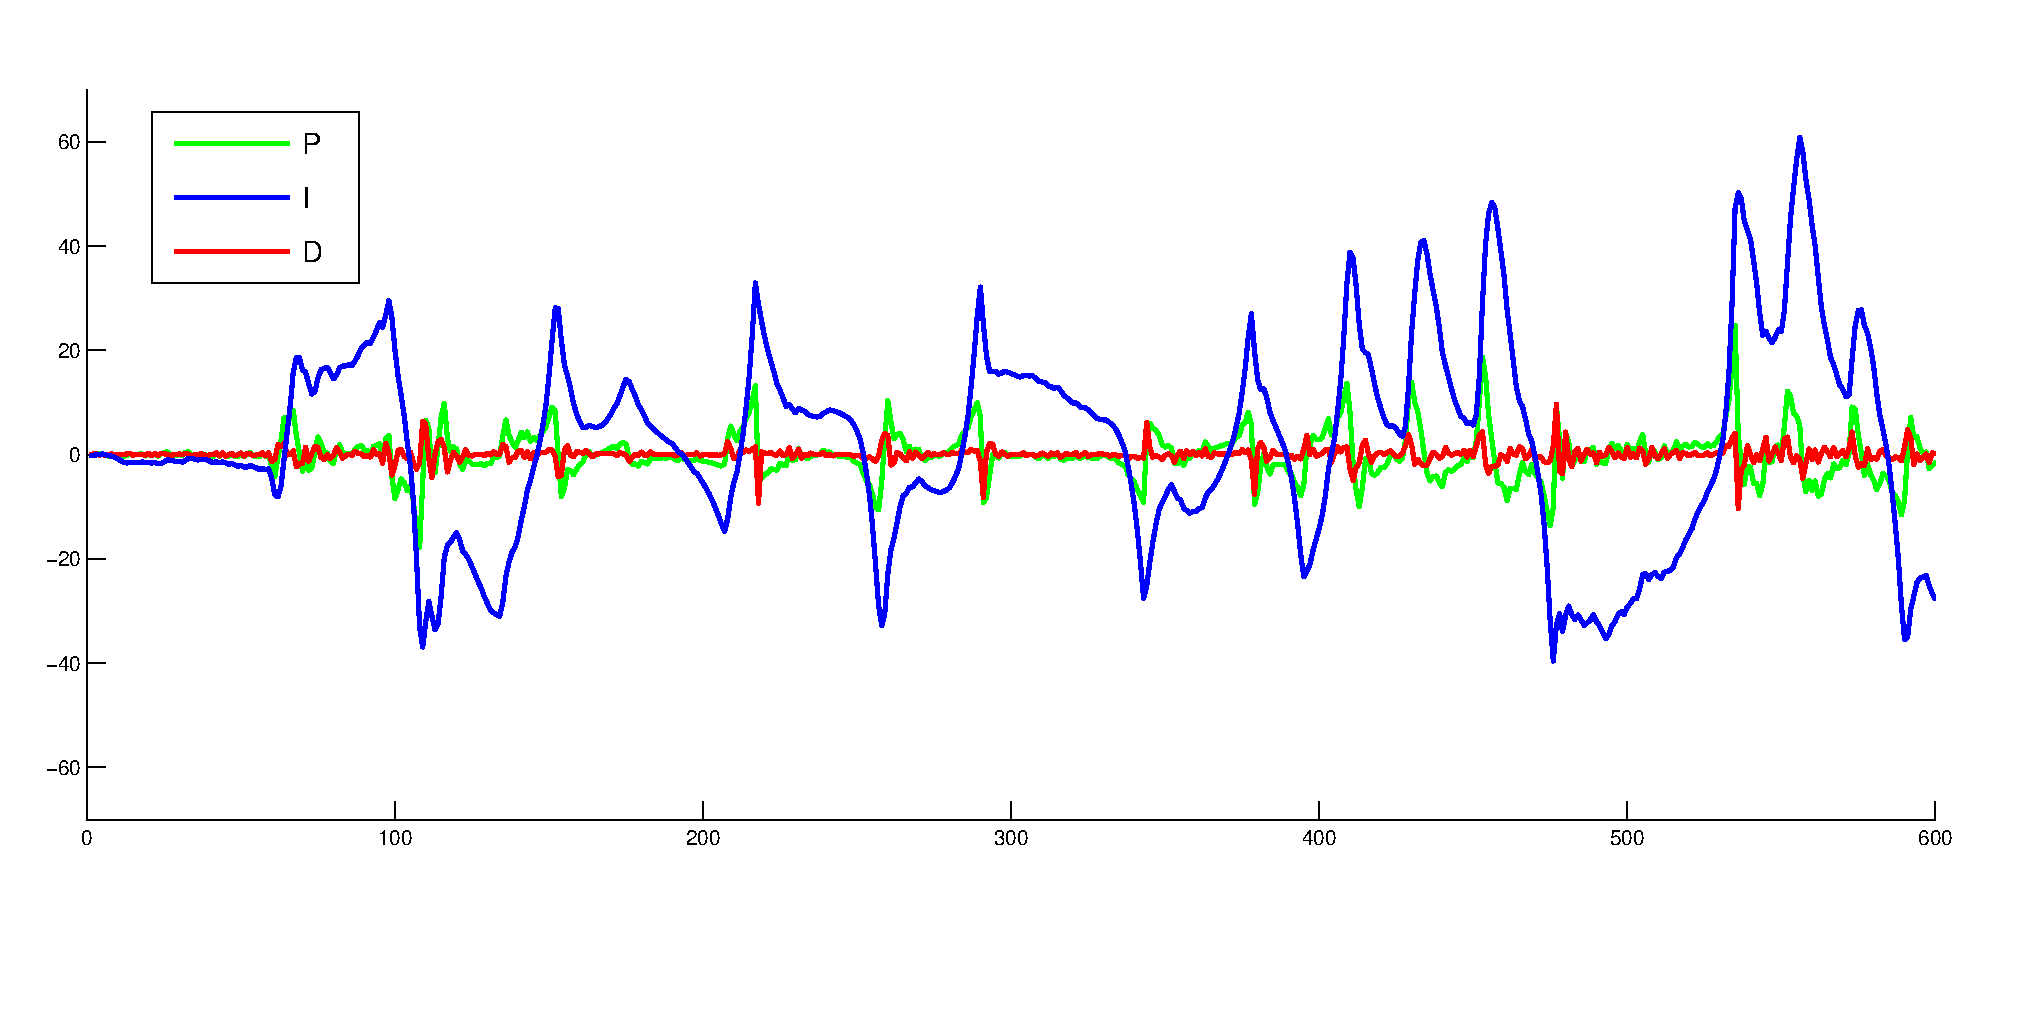
\includegraphics[width=1\linewidth]{images/pid.eps}
	\captionsetup{justification=centering,margin=1.5cm}
	\caption[Egy tesz során kapott PID tagjainak értékeit ábrázolja]
	{Egy tesz során kapott PID tagjainak értékeit ábrázolja. Az x tengelyen jelöljük a iterációk számát,	az y tengelyen a PID tagok értékének mértékét.}
	\label{pidFig}
\end{figure}

\chapter{Megvalósítás}\label{ch:MEGVALOSITAS}
\begin{osszefoglal}
	A projekt egy EV3 készletből épített kétkerekű egyensúlyozó robot irányítását valósítja meg hálózaton keresztül, telefonos alkalmazáson segítségével. E fejezet alatt bemutatásra kerülnek a megvalósítás során felmerült problémák, ezek megoldása és a felhasznált technológiák.
\end{osszefoglal}
\section{EV3 programozása}\label{sec:MEGVALOSITAS:lejos}
A LEGO MINDSTORMS kifejlesztett egy programozási környezetet, mely célja, hogy a megépített robotot különböző funkcionalitásokkal lehessen felruházni. E környezet lehetővé teszi a kisebb korosztály számára is a robotok programozását. Különböző grafikus elemekből úgynevezett blokkokból épül fel a program, amely USB-n keresztül kitelepíthető az EV3 vezérlőegységen futó LEGO MINDSTORMS által fejlesztett firmware.
Az előbb említett programozási környezet nem alkalmas komplexebb problémák megoldására. Ezért több firmware-t is kifejlesztettek melyek magas szintű programozási nyelveket támogatnak. Esetünkben a leJOS firmware-t használjuk.

A leJOS firmware-t José Solórzano hozta létre 1999 végén és azóta is folyamatosan fejlesztik. Linux alapú, nyílt forráskódú, magába foglalja a JVM-t (Java virtual machine), a neve is rámutat a Java programozhatóságra JOS(Java Operating System). Lehetővé teszi, a robot programozását Java-ban, támogatja a objektum orientált programozást. Mindezek lehetővé teszik a socket alapú komunikációt, szinkronizálhatóságot, szálak alkalmazását, Java típusok használatát és támogatja az EV3 szenzorokat.

Annak érdekében, hogy az EV3 vezérlőegységen futtassuk és könnyedén kitelepitsük a programokat az Eclipse IDE fejlesztői környezetre van szükség és a leJOS plugin-ra.

Mivel az EV3 vezérlőegységen az alapértelmezett firmware van telepítve ezért külön SD kártyára felkel telepíteni a leJOS-t. Legalább 2GB-os SD kártya de ne legyen 32GB-nál nagyobb és ne SDXC típusú legyen, mert nem ismeri fel az EV3 hardware. Az SD kártyát szükséges formázni FAT32 típusú partícióra. A leJOS számítógépre való telepítése során szükség lesz az 1.7 JDK-ra(Java Development Kit). Az előkészített program segítségével feltelepíthető a leJOS firmware az SD kártyára, ehhez még kell a JRE(Java Runtime Environment) is. Sikeres telepítés után az SD kártyát behelyezve az EV3 vezérlőegységbe elindítható a firmware, ha az alapértelmezett rendszer indul el akkor megkel ismételni az SD kártyára való telepítést. Ezt követően telepítsük az Eclipse plugin-t majd berakjuk az EV3\_HOME-t környezeti változónak és a bin könyvtárat a path-be.

\section{Androidos alkalmazás és kommunikáció}\label{sec:MEGVALOSITAS:android}
A projekt része egy telefonos alkalmazás, mely célja hogy hálózaton keresztül kapcsolódjon a robothoz és kommunikáljon vele. Az alkalmazás Android stúdióba készítettük és a kommunikációt java socketen keresztül valósítottuk meg, amit a leJOS, Linux alapú firmware tesz lehetővé.

Az alkalmazást elindítva megadhatjuk a robot IP és PORT címét amin keresztül csatlakozik. A csatlakozás során ellenőrizzük a bekért adatok helyes formátumát és hogy lehetséges vagy sem a kapcsolat. Az alkalmazás kezelését elősegíti egy általunk létrehozott "Remember me" funkcionalitás, mely célja hogy a legutóbbi IP és PORT címet visszatöltse az alkalmazás élindításakor. E megvalósítása a SharedPreferences API-n keresztül történik, érték és kulcs párok alapján tárolódnak fájlba az adatok. Ezen adatok hozzáférési pontja a SharedPreferences objektum, amely könnyen kezelhető metódusokat biztosít ezek olvasására illetve írására.

A sikeres kapcsolódást követően egy 2D-s joystick segítségével lehet irányítani a robotot négy irányba. A joystick vizuális megjelenítésére két kört rajzolunk ki a telefon képernyőjére canvas segítségével, amely felületéhez hozzárendeljük a megfelelő eseményfigyelőt(OnTouchListener). Annak érdekében, hogy a felhasználó ne tudja kimozdítani a nagyobb körön belüli kisebb kört átalakításokat végzünk koordináták között.

A képernyőt megérintve az eseményfigyelő által megkapjuk az $x$ és $y$ koordinátákat, ezeket a pontokat átalakítjuk polárkoordinátákba: $$(x,y) \Longrightarrow (r,\varphi)$$ $$r=\sqrt{x^2+y^2}$$ $$\varphi=arctg(y,x)$$ Tudva a két kör sugarának különbségét és a polárkoordinátákat, leellenőrizhető hogy a kis kör nagy kör sugarán kívül esik vagy sem. Abban az esetben ha a nagy körön kívül esik a kirajzolási pont, akkor a sugár mentén rajzoljuk ki a kisebb kört a szög függvényében. Ehhez szükséges polárkoordinátából átalakítani euklideszi koordinátába:  $$(r,\varphi) \Longrightarrow (x,y)$$ $$x=R*cos(\varphi)$$ $$y=R*sin(\varphi),$$ ahol R a két kör sugarának különbsége.

Tudva a mozgatás irányát, socketen keresztül küldjük a megfelelő adatokat. Az adatok szerializációját illetve titkosítását a Google Protocol Buffers által biztosítjuk, amely lehetővé teszi, hogy megszerkesszük az adatok struktúráját majd egy speciális generátorral létrehozzuk ezen strukturált adatok kezelésére a hozzá tartozó Java osztályt. E létrehozott osztályon keresztül könnyedén kezelhetjük a strukturált adatokat.

A Google Protocol Buffers használatához létre kell hozzunk egy \texttt{.proto} \ref{gpb} kiterjesztésű állományt, amelyben definiáljuk az adataink struktúráját. Az állomány első sorában deklaráljuk a csomag(package) nevét, második sorban konkrétan megadjuk a Java csomag hierarchiáját és a harmadik sorban megadjak az osztály nevet, amellyel rendelkezni fog a legenerált osztály. Abban az esetben ha nem adunk meg konkrét nevet a \texttt{java\_outer\_classname} mezőben akkor a \texttt{.proto} fájl nevét fogja megkapni. A további sorokban megadjuk az adattagokat, amelyek rendelkeznek típus névvel ez lehet bool, int32, float, double és string. Minden attribútumnak megadunk egy számot, amely egyedi azonosítóként szerepel a bináris kódolás során. Ezeken kívül megadható három típus mező minden attribútumnak, amelyek a következők: \texttt{required, optional, repeated}. A \texttt{required} mezővel beállíthatjuk, hogy az adott attribútum kötelezően értéket kapjon különbem RuntimeException vagy IOException hibát eredményez.  A \texttt{optional} mezőt annak az adattagnak állítjuk be, amely nem biztos, hogy értéket kap futási időben, ebben az esetben megadhatunk \texttt{.proto} állományban egy alapértelmezett értéket ennek az adattagnak. A \texttt{repeated} típussal lehetséges annak a jelzése, hogy az adott adattag ismétlődni fog.

\lstinputlisting[label=gpb,caption= Az adatok strukturáját definiáló .proto állomány, language=Java]{progfiles/dataProtos.proto}






 

%\chapter{Robot programozása}\label{ch:PROG}
\section{Mindstorms}\label{sec:PROG:mindstorms}
\section{leJOS keretrendszer}\label{sec:PROG:lejos}
%\chapter{Kommunikáció és irányítás}\label{ch:KONTROLLER}
\section{Megvalósítása}\label{sec:KONTROLLER:megvalositas}
\section{Android applikáció}\label{sec:KONTROLLER:app}
\section{Protocol Buffers}\label{sec:KONTROLLER:protobuff}

%\include{fejleszthetoseg}
\appendix

{ 
	\renewcommand{\baselinestretch}{1.1}\normalsize %
	\setlength{\itemsep}{-2.4mm}
	\setlength{\bibspacing}{0.67\baselineskip}
	\bibliographystyle{abbrvnat_hu}
	\bibliography{dolgozat}
}


\end{document}
